\documentclass[times]{itmo-student-thesis}

%% Опции пакета:
%% - specification - если есть, генерируется задание, иначе не генерируется
%% - annotation - если есть, генерируется аннотация, иначе не генерируется
%% - times - делает все шрифтом Times New Roman, собирается с помощью xelatex
%% - languages={...} - устанавливает перечень используемых языков. По умолчанию это {english,russian}.
%%                     Последний из языков определяет текст основного документа.

%% Делает запятую в формулах более интеллектуальной, например:
%% $1,5x$ будет читаться как полтора икса, а не один запятая пять иксов.
%% Однако если написать $1, 5x$, то все будет как прежде.
\usepackage{icomma}

%% Один из пакетов, позволяющий делать таблицы на всю ширину текста.
\usepackage{tabularx}

\usepackage{xspace}

\usepackage{graphicx}
\graphicspath{{imgs/}}
\DeclareGraphicsExtensions{.png,.jpg}

\newcommand{\alglambda}{${(1 + (\lambda , \lambda))}$\xspace}
\newcommand{\alglambdaf}{${(1 + (\lambda , \lambda))}$-ГА\xspace}


\newcommand{\oea}{\mbox{$(1 + 1)$-ЭА}\xspace}
\newcommand{\oplea}{\mbox{$(1+\lambda)$-ЭА}\xspace}
\newcommand{\mpoea}{\mbox{$(\mu+1)$-ЭА}\xspace}
\newcommand{\mplea}{\mbox{$(\mu+\lambda)$-ЭА}\xspace}
\newcommand{\mclea}{\mbox{$(\mu,\lambda)$-ЭА}\xspace}
\newcommand{\oclea}{\mbox{$(1,\lambda)$-ЭА}\xspace}
\newcommand{\ollga}{${(1 + (\lambda , \lambda))}$-ГА\xspace}

\newcommand{\onemax}{\textsc{OneMax}\xspace}
\newcommand{\leadingones}{\textsc{LeadingOnes}\xspace}
\newcommand{\om}{\textsc{OM}\xspace}
\newcommand{\jump}{\textsc{Jump}\xspace}
\newcommand{\N}{{\mathbb N}}
\newcommand{\R}{{\mathbb R}}
\newcommand{\eps}{\varepsilon}

\renewcommand{\binom}[2]{\mbox{$C^{#2}_{#1}$}}

\DeclareMathOperator{\Bin}{Bin}
\DeclareMathOperator{\Geom}{Geom}
\DeclareMathOperator{\pow}{pow}
\DeclareMathOperator*{\argmax}{arg\,max}
\DeclareMathOperator*{\argmin}{arg\,min}
%% Данные пакеты необязательны к использованию в бакалаврских/магистерских
%% Они нужны для иллюстративных целей
%% Начало
\usepackage{tikz}
\usetikzlibrary{arrows}
\usepackage{filecontents}
\begin{filecontents}{bachelor-thesis.bib}
@article{DoerrDE15,
  author = {Benjamin Doerr and
Carola Doerr and
Franziska Ebel},
  title = {From black-box complexity to designing new genetic algorithms},
  year = {2015},
  journal = {Theoretical Computer Science},
  optdoi = {10.1016/j.tcs.2014.11.028},
  optissn = {0304-3975},
  optnote = {Preliminary version in Proc.~of GECCO 2013},
  opturl = {http://dx.doi.org/10.1016/j.tcs.2014.11.028},
  pages = {87--104},
  volume = {567},
  langid = {english}
}

@article{DoerrD18,
  author = {Benjamin Doerr and Carola Doerr},
  title = {Optimal static and self-adjusting parameter choices for the (1+({\(\lambda\)},
{\(\lambda\)})) genetic algorithm},
  year = {2018},
  journal = {Algorithmica},
  optnumber = {5},
  pages = {1658--1709},
  volume = {80},
  langid = {english}
}

@online{ doerr-doerr-lambda-lambda-self-adjustment-arxiv,
    year        = {2019},
    title       = {Optimal Parameter Choices Through Self-Adjustment: Applying the 1/5-th Rule in
                   Discrete Settings},
    author      = {Benjamin Doerr and Carola Doerr},
    url         = {http://arxiv.org/abs/1504.03212},
    year        = {2015},
    langid      = {english}
}

@inproceedings{ example-english,
    year        = {2015},
    booktitle   = {Proceedings of IEEE Congress on Evolutionary Computation},
    author      = {Maxim Buzdalov and Anatoly Shalyto},
    title       = {Hard Test Generation for Augmenting Path Maximum Flow
                   Algorithms using Genetic Algorithms: Revisited},
    pages       = {2121-2128},
    langid      = {english}
}

@article{ example-russian,
    author      = {Максим Викторович Буздалов},
    title       = {Генерация тестов для олимпиадных задач по программированию
                   с использованием генетических алгоритмов},
    journal     = {Научно-технический вестник {СПбГУ} {ИТМО}},
    number      = {2(72)},
    year        = {2011},
    pages       = {72-77},
    langid      = {russian}
}

@article{ unrestricted-jump-evco,
    author      = {Maxim Buzdalov and Benjamin Doerr and Mikhail Kever},
    title       = {The Unrestricted Black-Box Complexity of Jump Functions},
    journal     = {Evolutionary Computation},
    year        = {2016},
    note        = {Accepted for publication},
    langid      = {english}
}

@book{ bellman,
    author      = {R. E. Bellman},
    title       = {Dynamic Programming},
    address     = {Princeton, NJ},
    publisher   = {Princeton University Press},
    numpages    = {342},
    pagetotal   = {342},
    year        = {1957},
    langid      = {english}
}
\end{filecontents}
%% Конец

%% Указываем файл с библиографией.
\addbibresource{bachelor-thesis.bib}

\begin{document}

\studygroup{M3435}
\title{Анализ генетического алгоритма (1 + (лямбда, лямбда)) на задаче максимального разреза графа}
\author{Черноокая Виктория Александровна}{Черноокая В.А.}
\supervisor{Антипов Денис Сергеевич}{Антипов Д.С.}{PhD}{}
\publishyear{2022}
%% Дата выдачи задания. Можно не указывать, тогда надо будет заполнить от руки.
\startdate{01}{сентября}{2018}
%% Срок сдачи студентом работы. Можно не указывать, тогда надо будет заполнить от руки.
\finishdate{31}{мая}{2019}
%% Дата защиты. Можно не указывать, тогда надо будет заполнить от руки.
%%\defencedate{15}{июня}{2019}

%%\addconsultant{Белашенков Н.Р.}{канд. физ.-мат. наук, без звания}
%%\addconsultant{Беззубик В.В.}{без степени, с велкиим званием}

\secretary{Павлова О.Н.}

%% Задание
%%% Техническое задание и исходные данные к работе
\technicalspec{Требуется разработать стилевой файл для системы \LaTeX, позволяющий оформлять бакалаврские работы и магистерские диссертации
на кафедре компьютерных технологий Университета ИТМО. Стилевой файл должен генерировать титульную страницу пояснительной записки,
задание, аннотацию и содержательную часть пояснительной записк. Первые три документа должны максимально близко соответствовать шаблонам документов,
принятым в настоящий момент на кафедре, в то время как содержательная часть должна максимально близко соответствовать ГОСТ~7.0.11-2011
на диссертацию.}

%%% Содержание выпускной квалификационной работы (перечень подлежащих разработке вопросов)
\plannedcontents{Пояснительная записка должна демонстрировать использование наиболее типичных конструкций, возникающих при составлении
пояснительной записки (перечисления, рисунки, таблицы, листинги, псевдокод), при этом должна быть составлена так, что демонстрируется
корректность работы стилевого файла. В частности, записка должна содержать не менее двух приложений (для демонстрации нумерации рисунков и таблиц
по приложениям согласно ГОСТ) и не менее десяти элементов нумерованного перечисления первого уровня вложенности (для демонстрации корректности
используемого при нумерации набора русских букв).}

%%% Исходные материалы и пособия
\plannedsources{\begin{enumerate}
    \item ГОСТ~7.0.11-2011 <<Диссертация и автореферат диссертации>>;
    \item С.М. Львовский. Набор и верстка в системе \LaTeX;
    \item предыдущий комплект стилевых файлов, использовавшийся на кафедре компьютерных технологий.
\end{enumerate}}

%%% Цель исследования
\researchaim{Разработка удобного стилевого файла \LaTeX
             для бакалавров и магистров кафедры компьютерных технологий.}

%%% Задачи, решаемые в ВКР
\researchtargets{\begin{enumerate}
    \item обеспечение соответствия титульной страницы, задания и аннотации шаблонам, принятым в настоящее время на кафедре;
    \item обеспечение соответствия содержательной части пояснительной записки требованиям ГОСТ~7.0.11-2011 <<Диссертация и автореферат диссертации>>;
    \item обеспечение относительного удобства в использовании~--- указание данных об авторе и научном руководителе один раз и в одном месте, автоматический подсчет числа тех или иных источников.
\end{enumerate}}

%%% Использование современных пакетов компьютерных программ и технологий
\addadvancedsoftware{Пакет \texttt{tabularx} для чуть более продвинутых таблиц}{\ref{sec:tables}, Приложения~\ref{sec:app:1}, \ref{sec:app:2}}
\addadvancedsoftware{Пакет \texttt{biblatex} и программное средство \texttt{biber}}{Список использованных источников}

%%% Краткая характеристика полученных результатов
\researchsummary{Получился, надо сказать, практически неплохой стилевик. В 2015--2018 годах
его уже использовали некоторые бакалавры и магистры. Надеюсь на продолжение.}

%%% Гранты, полученные при выполнении работы
\researchfunding{Автор разрабатывал этот стилевик исключительно за свой счет и на
добровольных началах. Однако значительная его часть была бы невозможна, если бы
автор не написал в свое время кандидатскую диссертацию в \LaTeX,
а также не отвечал за формирование кучи научно-технических отчетов по гранту,
известному как <<5-в-100>>, что происходило при государственной финансовой поддержке
ведущих университетов Российской Федерации (субсидия 074-U01).}

%%% Наличие публикаций и выступлений на конференциях по теме выпускной работы
\researchpublications{По теме этой работы я (к счастью!) ничего не публиковал.
\begin{refsection}
Однако покажу, как можно ссылаться на свои публикации из списка литературы:
\nocite{example-english, example-russian}
\printannobibliography
\end{refsection}
}

%% Эта команда генерирует титульный лист и аннотацию.
\maketitle{Бакалавр}

%% Оглавление
\tableofcontents

%% Макрос для введения. Совместим со старым стилевиком.
\startprefacepage
В Главе 1 подробно описывается область исследования, которая включает в себя описание алгоритма \alglambdaf, задачи поиска максимального разреза графа.
Далее, в Главе 2 приводится теоретическая оценка предложенного алгоритма на полных графах, а также сравнение с ожидаемым временем работы других эволюционных алгоритмов.
В Главе 3 описываются результаты выполнения известных эволюционных алгоритмов, включая \alglambdaf на полных, полных двудольных и случайных графах, а также их сравнение.

%% Начало содержательной части.
\chapter{Применение генетического алгоритма \alglambda на задаче поиска максимального разреза графа}

%% Так помечается начало обзора.
\startrelatedwork
В данной главе описывается алгоритм \alglambda и постановка исследуемой задачи, а именно поиска максимального разреза графа.
Также сформулированны условия для получения теоретической и эмпирической оценки применения алгоритма \alglambda на задаче максимального разреза графа.
%% Так помечается конец обзора.
\finishrelatedwork

\section{Генетический алгоритм \alglambda}

Генетический алгоритм \alglambda~--- относительно недавно сформулированный эволюционный алгоритм, минимизирующий функцию приспособленности $f(x)~:~\{0, 1\}^n \rightarrow \R$ и содержайщий в себе 3 главных параметра:
\begin{itemize}
   \item размер популяции $\lambda \in \N$;
   \item вероятность мутации $p \in [0, 1]$;
   \item смещённость скрещивания $c \in [0, 1]$.
\end{itemize}
\alglambdaf работает с одной родительской особью $x$, которая инициализируется случайной битовой строкой длины $n$, где $n$ - размер проблемы. Затем проходят итерации, каждая из которых состоит из двух фаз: мутации и скрещивания(или кроссовера). На этапе мутации алгоритм сначала выбирает силу мутации $\ell$ из биномиального распределения $\Bin(n, p)$ с $n$ испытаниями и вероятностью успеха $p$. В алгоритме в фазе мутации \oea мы имеем $p = \frac{1}{n}$, но поскольку мы стремимся к более быстрому результату, то обычно рассматривают вероятность $p$, превышающую $\frac{1}{n}$.
После этого создается $\lambda$ потомков, каждый путем инвертирования $\ell$ случайных бит родителя. То есть выбираем набор из $ell$ различных позиций в $[n]$ случайным образом и создаем потомка, перевернув битовые значения в этих позициях.
Все эти потомки находятся на одинаковом расстоянии от родителя.
На промежуточном этапе отбора потомок с наименьшим значением функции приспособленности выбирается победителем мутации для дальнейшего участия в фазе скрещивания. Если таких несколько, то победитель выбирается равномерно случайным образом.
Обозначим этого потомка как $x'$.
Далее следует фаза скрещивания. Снова создается $\lambda$ потомков. На это раз каждый бит потомка берется из победителя мутации с вероятностью $c$ и из родителя с вероятностью $1 - c$. Победитель скрещивания $y$ получается тем же способом, как и на фазе мутации. В конце итерации происходит отбор или фаза выбора, где происходит сравнение значений функции приспособленности родителя $x$ и победителя скрещивания $y$.
Родитель заменяется особью-победителем $y$ фазы скрещивания, если значение $f(y)$ не больше $f(x)$. Псевдокод алгоритма представлен в Листинге 1.

\begin{algorithm}[h]
\caption{Псевдокод \alglambdaf, минимизирующего $f$}\label{ollgaMin}
\begin{algorithmic}
	\State$x \gets $ \textsc{случайная последовательность бит длины} $n$
	\For{$t \gets [1, 2, 3...]$}
		\State \textsc{Выбрать} $\ell$ \textsc{из} $\Bin\left(n, p\right)$ \Comment Фаза мутации
      		\For{$i \in [1..\lambda]$}
         		\State$x^{(i)} \gets$ \textsc{копия} $x$ \textsc{с инвертированными} $\ell$ \textsc{битами, взятыми из равномерного распределения}
         	\EndFor
	     	\State $x' \gets \argmin_{z \in \{x^{(1)}, \dots, x^{(\lambda)}\}}f(z)$

		\For{$i \in [1..\lambda]$} \Comment Фаза срещивания
	          	\State $y^{(i)} \gets$ \textsc{каждый бит с вероятностью $c$ берётся из $x'$ иначе из $x$}
		\EndFor
	      	\State $y \gets \argmin_{z \in \{y^{(1)}, \dots, y^{(\lambda)}\} }f(z)$

		\If{$f(y) \le f(x)$} \Comment Отбор
			\State $x \gets y$
		\EndIf
	\EndFor
\end{algorithmic}
\end{algorithm}

Алгоритм зависит от размера популяции $\lambda \in \N$, и вероятностей мутации и скрещивания $p, c \in [0, 1]$.
Без доказательства заметим, что алгоритм не сходится к оптимальному решению, когда $p = 0$ или $c = 0$, или $p = c = 1$.
Для всех остальных случаев он в конце концов находит (и сохраняет) оптимум.
При $c = 1$ на фазе скрещивания получается победитель мутации, что исключает влияние фазы кроссовера и \alglambdaf сводится к \oplea.
В частности, для $c = 1, p = \frac{1}{n} и \lambda = 1$ алгоритм является уже упомянутым \oea.
Во всех остальных случаях $0 < c < 1$ результат алгоритма \alglambdaf зависит от фазы скрещивания.
Поскольку для многих эволюционных алгоритмов, основанных на мутациях, вероятность мутации $\frac{1}{n}$ является рекомендуемым выбором~\cite{ссылка} (и иногда доказуемо оптимальным~\cite{ссылка}), то следует использовать алгоритм \alglambda с $p, c$, удовлетворяющим $pc = \frac{1}{n}$.
Из интуитивных соображений в ~\cite{ссылка} было предложено использовать такое соотношение параметров размера задачи $n$ и размера популяции $\lambda$:
\begin{itemize}
 \item $p = \frac{\lambda}{n}$;
 \item $c = \frac{1}{\lambda}$.
 \end{itemize}
Также такое соотношение параметров показало свою эффективность и было оптимальным на других анализируемых задачах, таких как \onemax~\cite{ссылка}, \leadingones~\cite{ссылка} и MAX-3SAT~\cite{ссылка}). В данной работе также будем исспользовать предложенные соотношения параметров.


\section{Задача о максимальном разрезе графа}

Смысл задачи о максимальном разрезе графа - для заданного неориентированного графа без петель и паралельных ребер $G = (V, E)$ с множеством вершин $V$ и ребер $E$ разбить множество вершин на 2 непересекающихся подмножества $V_1$ и $V_2$ так, что количество <<разрезанных>> ребер максимально и $V_1 \cup V_2 = V$.
Ребро $(v, u) \in E$ назвается <<разрезанным>>, если инцидентные ему вершины находятся в разных подмножествах $V_1$ и $V_2$, то есть $v \in V_1 \cap u \in V_2$ или $v \in V_2 \cap u \in V_1$.

$P$ - разбиение множества $V$ на 2 подмножества $V_1$ и $V_2$.
Представим его в виде битовой строки, где $i$-ый бит равен нулю, если $v_i \in V_1$, и единице, если $v_i \in V_2$.
Определим функцию  $Cut$ от разбиения $P$ :
\begin{align*}
   Cut(P) = |\{e = (v_1, v_2) \in E ~:~ v_1 \in V_1 \cap v_2 \in V_2\}|.
\end{align*}
Неформально говоря, это количество <<разрезанных>> ребер.

Задача является $NP$-трудной, что в текущих реалиях означает, что не существует детерминированного алгоритма, решающего задачу за полиномиальное время. Поэтому используются эволюционные алгоритмы.
Обычно это нетривиальная задача, так как мы не можем заранее знать сколько ребем мы можем <<разрезать>>. Например, для полного графа $K_n$ с четным $n$ оптимальным разбиение является то, которое разбивает вершины на два подмножества размером $\frac{n}{2}$. В этом случае мы разрезаем $\frac{n^2}{4}$ ребер, что чуть больше половины всех $\frac{n(n-1)}{2}$ ребер.

В рамках этой работы функцию приспособленности определим как
\begin{align*}
   f(x) = E - 2Cut(x),
\end{align*}
где x - разбиение, и будем считать, что разрез найден, если разрезана хотя бы половина ребер.
Это позволит нам получить хоть какую-то оценку эволюционных алгоритмов, а также для многих частных случаев является приближенным значением. Ранее уже проводились исследования работы других эволюционных алгоритмов на данной задаче с таким условием остановки, но для алгоритма \alglambdaf результатов ожидаемого времени работы еще получено не было.

\chapterconclusion
В данной главе был сформулирован алгоритм \alglambda, а также задача используемая для анализа времени работы на нем. Сформулированны и предложены оптимальные параметры для генетического алгоритма, а также затронуто сравнение реализации \alglambda с другими существующими эволюционными алгоритмами.

\chapter{Теоретическая оценка времени работы алгоритма}

\section{Анализ существующих алгоритмов}

\section{Анализ алгоритма \alglambda на полных графах}

\begin{lemma}\label{lem:mut1}
С вероятностью $1- o(1)$ хотя бы $\frac{\lambda}{8}$ инвертированных бит в каждой особи - это $0$, инвертированные в $1$.
\end{lemma}

\begin{proof}
Рассмотрим одну итерацию фазы мутации. $\ell$ - сила мутации, $x'$ - особь победителя, $B' = \{i \in [n] ~|~ x_i = 0 \cap x'_i = 1\}$ - набор битов, которые стали единицами из нулей.
Так как $\lambda = \omega(1)$ и $\ell$ из $\Bin\left(n, \frac{\lambda}{n}\right)$, то простое применение границ Чернова~\cite{ссылка} говорит, что $|\ell - \lambda| \le \frac{\lambda}{2}$ с вероятностью $1- o(1)$, то есть $\ell \in [\frac{\lambda}{2}, \frac{3\lambda}{2}]$.

Определим $d = d(x)$ - количество нулей в разбиении $x$. Проанализируем генерацию одного из $\lambda$ потомств. $B_1 = \{i \in [n] ~|~ x_i = 0 \cap x^{(1)}_i = 1\}$. Тогда снова используя границы Чернова, но для гипергеометрического распределения $HG(d, n, \ell)$~\cite{ссылка}, получим $Pr[|B_1| \ge \frac{d\ell}{2n}] = 1 - o(1)$.
Так как все потомки имеют одинаковое расстояние Хэмминга от $x$, а победитель мутации всегда особь с максимальным $B_1$, то $|B'| \ge |B_1| \ge \frac{d\ell}{2n} \ge \frac{\ell}{4}$. Учитывая ограничения, полученные для $\ell$, $Pr[|B'| \ge \frac{\lambda}{8}] = 1 - o(1)$.
\end{proof}\qed

\begin{lemma}\label{lem:mut2}
Вероятность, что из победителя мутации будет взято хотя бы $\frac{c\lambda}{log\lambda}$ бит равна $\Omega(1)$
\end{lemma}

\begin{proof}

\end{proof}
\chapterconclusion

В этой главе была получена верхняя оценка математического ожидания времени работы алгоритма \alglambda на задаче разреза половины ребер на полных графах $\mathbb{E}[T]=O(nlog(\lambda))$. Также было проведено сравнение теоретического результата ожидаемого времени работы \alglambdaf с другими эволюционными алгоритмами на задаче максимального разреза графа. Исходя из полученных данных для этой задачи, можно сделать вывод, что применение этого алгоритма менее эффективно, чем RLS и \oea.
\chapter{Эмпирическая оценка времени работы алгоритма для всех типов графов}
В этой главе рассматривается эмпирическая оценка времени работы алгоритма \alglambda на задаче максимального разреза графа для разных типов графов, описываются конфигурации тестовых запусков. В заключении прилагаются результаты экспериментов в виде графиков, а также анализ полученных данных.

\section{Конфигурации тестовых запусков}
Эксперименты, а также последующее сравнение результатов проводились для следующих алгоритмов:
\begin{itemize}
 \item \alglambdaf;
 \item \oea со стандартным операттором мутации;
 \item \oea с выбором вероятности по степенному закону;
 \item Random Local Search.
\end{itemize}
Алгоритмы запускались и начинали свою работу на графах, у которых разбиение было представлено битовой строкой только из нулей, то есть на первой итерации всех алгоритмов количество <<разрезанных>> ребер было равно нулю и все вершины находились в подмножестве $V_1$, согласно определению разбиения. Алгоритмы останавливали свою работу когда функция приспособленности достигала значения меньше либо равное нулю. То есть хотя бы половина ребер разрезана.
Эксперименты проводились на различных типах графов без петель и параллельных ребер:
\begin{itemize}
 \item полные графы;
 \item полные двудольные графы;
 \item случайно сгенерированные.
\end{itemize}
Также тестовые запуски проводились на графах с различным количеством вершин, равным степеням двойки: $2^5$, $2^6$, $2^7$, $2^8$, $2^9$, $2^{10}$, $2^{11}$.
В двудольных графах количество ребер в долях было одинаковым.

Для каждой конфигурации алгоритмы запускались по 80 раз для более точного анализа ожидаемого времени работы. Время работы считалось, как количество вычислений функции приспособленности. Конечным результатом времени работы алгоритма для каждого типа графа считалось среднее арифметическое результатов времени работы всех 80 запусков. Для отображения полученных значений на графиках таже учитывались отклонения от среднего.

Для алгоритма \oea с выбором вероятности по степенному закону константный параметр $\beta$ равен $1,5$. Для \alglambda используем константное значение $\lambda = 10$.
Решение об использовании именно этой константы было принято на основании дополнительных экспериментов проведенных на полных графов с количеством вершин - 1024. Для исследования рассматривались $\lambda$ равные 2, 4, 8, 16, 32, 64, 128. Для каждой лямбды алгоритм запускался также по 80 раз.

\begin{figure}[t!]
\center{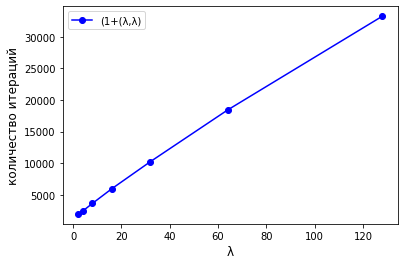
\includegraphics[scale=1]{Lambda}}
\caption{Производительность \ollga для различных значений $\lambda$ на полных графах с количеством вершин $2^{10}$}
\label{fig:lambda}
\end{figure}

На Рисунке~\ref{fig:lambda} изображен график зависимости числа вычислений функции приспособленности от значий $\lambda$. Исходя из графика можно сделать вывод, что брать большую $\lambda$ не оптимально, но и в случае слишком маленького значения, например равной 1, алгоритм не будет отличаться от \oea. Тогда, чтоб была возможность оценить эффективность данного генетического алгоритма выберем $\lambda = 10$. Для всех запусков \alglambdaf использовалась именно эта константа.

Для каждого запуска на каждой итерации собиралась и записывалась  информация:
\begin{itemize}
 \item текущее значение функции приспособленности $f$;
 \item значение $f$ для победителя мутации;
 \item значение $f$ для победителя кроссовера (для \alglambdaf).
\end{itemize}



\section{Результаты экспериментов}

\chapterconclusion
Также на основании полученных результатов проведенных экспериментов можно предполагать, что ожидаемое время работы для разных типов графов такое же как и для полных и равно $O(nlog(\lambda))$.

%% Макрос для заключения. Совместим со старым стилевиком.
\startconclusionpage

В данном разделе размещается заключение.

\printmainbibliography

%% После этой команды chapter будет генерировать приложения, нумерованные русскими буквами.
%% \startappendices из старого стилевика будет делать то же самое
\appendix

\chapter{Исходный код}\label{sec:app:1}

\end{document}
